\documentclass{ieeeaccess}
\usepackage{cite}
\usepackage{amsmath,amssymb,amsfonts}
\usepackage{algorithmic}
\usepackage{graphicx}
\usepackage{textcomp}
\usepackage{booktabs}
\usepackage{url}

% ---- IEEE Access blue: headings, captions, title, abstract label ---------
% ieeeaccess.cls sets accessblue up as PANTONE 3015 C, a *spot* colour, via
% the spotcolor package, and paints the paper title, section headings, the
% ABSTRACT / INDEX TERMS labels, and the FIGURE / TABLE caption labels with
% it. A spot colour is a printing construct: it is written into the PDF as a
% /Separation colourspace, which renders only if the engine and the viewer
% both honour one. More to the point here, the name stays bound to
% spotcolor's own colour machinery, so the first package that reloads xcolor
% afterwards takes over \color, detaches accessblue from that machinery, and
% every one of those \color{accessblue} calls quietly comes out black.
% \usepackage{tikz}, three lines below, is exactly such a package; pgfplots
% is another.
%
% Re-declaring the two colours as ordinary device colours, before those
% packages load, removes the dependency. The numbers are not guessed: they
% are the class's own alternate for PANTONE 3015 C, copied from the
% \AddSpotColor call above it in ieeeaccess.cls (1, 0.3, 0, 0.2) and from
% its greycolor definition. Nothing else about the class is touched --- the
% sectioning hooks, numbering, casing and spacing are all left alone.
\usepackage{xcolor}
\definecolor{accessblue}{cmyk}{1,0.3,0,0.2}
\definecolor{greycolor}{cmyk}{0,0,0,.8}
% --------------------------------------------------------------------------

\usepackage{tikz}
\usepackage{pgfplots}
\usetikzlibrary{arrows.meta,positioning}
\pgfplotsset{compat=1.18}
\graphicspath{{figures/},{paper/figures/},{assets/}}

% categorical slots 1-3 of the validated light-mode palette
\definecolor{dOne}{HTML}{2a78d6}
\definecolor{dTwo}{HTML}{eb6834}
\definecolor{dThree}{HTML}{1baf7a}

% ieeeaccess defines \headeretal; provide a fallback so the file compiles
% against any vintage of the class file.
\providecommand{\headeretal}{et al.}
\def\BibTeX{{\rm B\kern-.05em{\sc i\kern-.025em b}\kern-.08em
    T\kern-.1667em\lower.7ex\hbox{E}\kern-.125emX}}
\begin{document}
\history{Date of publication xxxx 00, 0000, date of current version xxxx 00, 0000.}
\doi{10.1109/ACCESS.2026.DOI}

\title{TabML-Guard: A Configuration-Driven Pipeline for Cost-Accounted Hyperparameter Optimization, Explainable Triage, and Concept-Drift Monitoring on Time-Ordered Tabular Data}

\author{\uppercase{Ayush Gole}\authorrefmark{1}, \uppercase{Sarvadnya Kakad}\authorrefmark{1}, and \uppercase{Sneha Annapanavar}\authorrefmark{2}}
\address[1]{Department of Computer Engineering, Vidyalankar Institute of Technology, Mumbai, India (e-mail: ayushgole1910@gmail.com, sarvadnya.kakad@vit.edu.in)}
\address[2]{Faculty, Department of Computer Engineering, Vidyalankar Institute of Technology, Mumbai, India (e-mail: sneha.annapanavar@vit.edu.in)}
\tfootnote{This work was carried out as part of the Advanced Machine Learning course project. The authors thank the maintainers of the open-source libraries on which this work depends.}

\markboth
{Gole \headeretal: TabML-Guard: Cost-Accounted HPO, Explainable Triage, and Drift Monitoring}
{Gole \headeretal: TabML-Guard: Cost-Accounted HPO, Explainable Triage, and Drift Monitoring}

\corresp{Corresponding author: Ayush Gole (e-mail: ayushgole1910@gmail.com).}

\begin{abstract}
Practitioners who build predictive models on time-ordered tabular data face four questions that a single accuracy figure cannot answer: is a boosting ensemble worth its complexity over a regularized linear model; does hyperparameter optimization justify the compute it consumes; which individual predictions should be escalated to a human; and will the model still work next quarter. We present TabML-Guard, a configuration-driven pipeline that answers these questions end to end and reports the answers in one self-contained document. From a short configuration file the pipeline ingests any tabular dataset, infers whether the task is classification or regression, and splits the rows temporally so the model always trains on the past and is tested on the future. It then fits regularized baselines, boosting ensembles, and a regularized stacking meta-model; compares default, grid, random, and Bayesian search at an equal evaluation budget while recording wall-clock cost alongside score; explains the winning model with SHAP and routes its least-confident predictions to human review; and monitors drift through walk-forward prequential evaluation, the Population Stability Index, and paired significance tests. We exercise the pipeline on three time-ordered datasets spanning both task types. The results are unflattering to conventional practice: regularization strength was almost inert, no model family won universally, tuning returned anything from an 18\% gain to a small loss depending on the dataset, and large input drift did not produce the performance decay it is usually assumed to cause. The system is released as open source.
\end{abstract}

\begin{keywords}
automated machine learning, concept drift, explainable artificial intelligence, gradient boosting, hyperparameter optimization, model reliability, tabular data
\end{keywords}

\titlepgskip=-15pt

\maketitle

\section{Introduction}
\label{sec:introduction}
\PARstart{T}{abular} data remains the workhorse of applied machine learning. Surveys of deployed systems consistently find that the majority of industrial prediction problems are still solved on structured, column-oriented data rather than images or text, and that the models doing the work are overwhelmingly gradient-boosted trees and regularized linear models \cite{shwartz2022tabular,grinsztajn2022tree}. The tooling around that work, however, has a well-documented failure mode. A model is trained once, in a notebook, for one dataset; the evaluation quietly assumes that the future is available at training time; a single accuracy number is reported; and nothing is said about whether the number will still hold next quarter \cite{sculley2015hidden,paleyes2022challenges}.

Four specific questions are routinely left unanswered, and each of them is answerable with modest effort:

\begin{enumerate}
\item \textbf{Is the ensemble earning its complexity?} It is now reflexive to reach for XGBoost, LightGBM, or CatBoost. On small, low-dimensional, noisy tables that reflex is frequently wrong, and the cost, in tuning time, inference latency, and operational surface, is paid regardless.
\item \textbf{Does tuning pay for itself?} Hyperparameter optimization is usually reported as an accuracy number, never as a ratio of gain to compute. A search that improves a metric by a third of a percent after fifteen minutes of CPU time is, in most deployment contexts, a net loss, and the practitioner has no way to see that from a leaderboard.
\item \textbf{Which predictions should a human check?} An accuracy of 78\% means that 22\% of predictions are wrong. It does not say which ones. A model that ``knows when it does not know'' can be operated very differently from one that fails uniformly.
\item \textbf{Will the model survive contact with time?} A model trained on the past is deployed into a future whose feature distributions may have moved. Whether that movement harms accuracy is an empirical question that a random train/test split cannot even pose.
\end{enumerate}

Existing automated machine learning (AutoML) systems answer the first question only as a by-product of maximizing a score, and are largely silent on the other three. auto-sklearn \cite{feurer2015auto}, Auto-WEKA \cite{kotthoff2013auto}, TPOT \cite{olson2016tpot}, and AutoGluon-Tabular \cite{erickson2020autogluon} all optimize predictive performance under a compute budget; they do not report the marginal value of that compute, they do not produce per-prediction triage, and they do not monitor the model after it has been handed over. Conversely, the concept-drift literature has mature methodology (prequential evaluation, change detection, windowed retraining \cite{gama2014survey,zliobaite2010learning}) but it is rarely packaged into the same artifact as model selection, and the data-science tooling that practitioners actually use rarely reaches for it.

This paper describes \textbf{TabML-Guard}, a system built to close that gap. It is an integration rather than a new algorithm. Its contribution is to make the honest version of the workflow the default, and to make the system's own conclusions, including the inconvenient ones, the primary output.

\subsection{Contributions}
The specific contributions are as follows.

\begin{itemize}
\item \textbf{C1. A configuration-driven, dataset-agnostic pipeline.} Every dataset-specific decision lives in a single YAML file. No module in the implementation names a dataset, and the same code path serves classification and regression by inferring the task from the target column. Generality is demonstrated rather than asserted: three datasets, two task types, and three feature regimes run through unchanged code.
\item \textbf{C2. Cost-accounted hyperparameter-optimization comparison.} Default, grid, random, and Bayesian search are compared at an \emph{equal evaluation budget} on the same cross-validation splitter, with wall-clock seconds and evaluation counts recorded next to the score. The system reports a verdict on whether tuning was worth its cost, and that verdict is permitted to be negative.
\item \textbf{C3. Temporal-honesty by construction.} Rows are split by time rather than shuffled, preprocessing statistics are learned inside every fold, and the held-out temporal test set is never touched during model selection, tuning, or the regularization sweep. Leakage is prevented structurally rather than by reviewer vigilance.
\item \textbf{C4. Triage rather than explanation alone.} Alongside SHAP attributions \cite{lundberg2017unified}, the pipeline implements a confidence-based reliability layer that routes the least-confident fraction of predictions to human review, and then \emph{measures whether the routing worked} by reporting the fraction of all errors it captured.
\item \textbf{C5. A deployable drift and significance study.} Walk-forward prequential monitoring races a frozen model against a retraining one, the Population Stability Index tracks input drift, and McNemar's test \cite{mcnemar1947note} or the Wilcoxon signed-rank test \cite{wilcoxon1945individual} adjudicates every ``model A beats model B'' claim.
\item \textbf{C6. An end-to-end report as the deliverable.} The output is a single self-contained document that leads with a plain-language verdict, so the analysis is legible to the person who owns the decision rather than only to the person who ran the code.
\end{itemize}

\subsection{Findings in brief}
Because the empirical results are the substance of this paper, we state them up front. On three time-ordered datasets: (i) the choice among $L_1$, $L_2$, and elastic-net penalties changed the held-out score by at most $0.02\%$, so regularization strength was a far weaker lever than is commonly assumed; (ii) no model family dominated: a regularized linear model won two of the three datasets and a tuned CatBoost model won the third, while on one dataset every boosting ensemble was catastrophically worse than a plain linear fit; (iii) the return on hyperparameter optimization ranged from $+18.2\%$ to $-0.7\%$ across the three datasets, at a cost that grew super-linearly; (iv) flagging the least-confident 20\% of predictions captured 34\% of all errors, and the auto-accepted remainder was 24 percentage points more accurate than the flagged slice; and (v) input distributions drifted heavily everywhere (mean PSI far beyond the conventional ``large shift'' threshold) yet measured performance did not decay on any dataset, and retraining helped only on the regression tasks.

\subsection{Organization}
Section~\ref{sec:related} reviews related work and sharpens the gap. Section~\ref{sec:method} describes the pipeline stage by stage. Section~\ref{sec:experiments} specifies the datasets, configurations, and metrics. Section~\ref{sec:results} reports results. Section~\ref{sec:discussion} discusses the findings, their threats to validity, and the limitations of the study. Section~\ref{sec:conclusion} concludes.

\section{Related Work}
\label{sec:related}

\subsection{Automated machine learning for tabular data}
AutoML systems search over preprocessing, model families, and hyperparameters to maximize a predictive metric. Auto-WEKA \cite{kotthoff2013auto} formulates model selection as a sequential model-based optimization problem; auto-sklearn \cite{feurer2015auto} adds meta-learning and ensemble construction; TPOT \cite{olson2016tpot} performs genetic-programming search over pipeline graphs; AutoGluon-Tabular \cite{erickson2020autogluon} combines a fixed set of strong learners through multi-layer stacking and reaches competitive accuracy with little search. These systems are excellent at what they set out to do, and TabML-Guard does not compete with them on accuracy. The difference is the objective. AutoML asks \emph{which pipeline scores highest}; TabML-Guard asks \emph{whether the gain was worth its cost, which predictions are untrustworthy, and whether the model still works}. Those are operational questions that a leaderboard does not answer, and in our experiments the two objectives even disagreed: on two of three datasets the AutoML-style answer, tuning the booster, produced a model that the untuned regularized baseline beat.

The observation that boosted trees dominate on tabular data is well established \cite{grinsztajn2022tree,shwartz2022tabular}, and it is the reason the ensemble layer exists here. Our results qualify it: the dominance is real on the larger, higher-cardinality dataset and absent on the two smaller ones, which is consistent with the finding that tree ensembles lose their edge as the signal-to-noise ratio falls.

\subsection{Regularization and ensemble stacking}
Ridge regression \cite{hoerl1970ridge} shrinks coefficients smoothly under an $L_2$ penalty; the lasso \cite{tibshirani1996lasso} drives some coefficients exactly to zero under an $L_1$ penalty and thereby performs embedded feature selection; the elastic net \cite{zou2005elastic} interpolates between them. Stacked generalization \cite{wolpert1992stacked} trains a meta-learner on out-of-fold predictions from a set of base learners. The most recent of the systems that informed this work, RegStack, argues that regularization belongs in both places, in the base learners and in the stacking meta-model, rather than being an afterthought \cite{regstack2025}. We adopt that position directly: the meta-learner in our stacking layer is always a regularized linear model, and the regularization path is a first-class diagnostic rather than a tuning nuisance.

\subsection{Hyperparameter optimization}
Grid search is exhaustive and combinatorial. Random search \cite{bergstra2012random} is the classic rebuttal: because only a few hyperparameters matter in practice, sampling configurations uniformly explores the effective space more efficiently per unit of compute. Sequential model-based methods, such as Bayesian optimization with a Gaussian-process or tree-structured Parzen surrogate, spend part of the budget learning a surrogate of the response surface and using it to propose the next configuration \cite{snoek2012practical}. Optuna \cite{akiba2019optuna} popularized the tree-structured Parzen estimator variant and made it accessible. Recent studies combining Bayesian optimization with gradient boosting architectures (such as BO-XGBoost \cite{boxgboost2026}) demonstrate strong empirical results on complex industrial tabular tasks. However, the empirical question of \emph{when} the surrogate's computational overhead is repaid in practice is contested, and the literature usually reports only the terminal score. Our third stage is a direct attempt to answer that question with the cost axis made explicit, in the spirit of the argument that parameter choice can matter as much as algorithm choice \cite{spectral2025}.

\subsection{Explainability and prediction reliability}
SHAP \cite{lundberg2017unified} unifies several attribution methods as Shapley values from cooperative game theory, providing additive, locally accurate attributions with desirable consistency properties. It has become the default post-hoc tool for tabular models. LIME \cite{ribeiro2016lime} takes a complementary local-surrogate approach. Both explain a prediction; neither, on its own, tells an operator which predictions to distrust.

That gap is addressed by a smaller literature on calibration and reliability. Reliability diagrams \cite{niculescu2005predicting,guo2017calibration} expose the gap between stated confidence and empirical accuracy; uncertainty-quantification methods \cite{gal2016dropout} estimate predictive variance. The most direct inspiration for our fourth stage is recent work showing that explanation signals can be used not merely to describe a model but to \emph{identify and compensate for} its unreliable predictions \cite{shapcomp2025}. We implement the identification half of that idea as a deployable routing rule and quantify its yield. The framing is that of human-in-the-loop triage rather than autonomous abstention \cite{settles2009active}.

\subsection{Concept drift}
Distribution shift over time is the defining hazard of deployed models. A substantial literature covers its taxonomy and detection: change detectors such as ADWIN maintain an adaptive window over an error stream and raise an alarm when the windowed mean shifts beyond a bound \cite{bifet2007adwin}; DDM and Page--Hinkley variants monitor classifier error directly; comprehensive surveys catalogue the space \cite{gama2014survey,zliobaite2010learning}. Prequential (test-then-train) evaluation is the standard protocol for measuring a learner on a stream without look-ahead. The Population Stability Index, long used in credit-risk scorecard monitoring \cite{siddiqi2005credit}, provides a cheap per-feature measure of covariate shift.

The dataset used as our primary classification case, ELEC2, is a standard drift benchmark, and the drift paper that motivated this work uses it to study streaming adaptation with continuous kernel learning \cite{drift2024}. We adopt its problem framing (streaming data, distribution change, ensemble adaptation) but implement the pragmatic monitor-and-retrain pattern its problem motivates rather than its continuous-kernel algorithm. That is a scope decision: the goal is the deployable pattern, and the results below show why the distinction matters, since heavy covariate shift in our experiments was not accompanied by the performance decay that a naive reading of the drift literature would predict.

\subsection{Positioning}
Table~\ref{tab:positioning} places TabML-Guard against the categories above. The distinguishing feature is that all of them are produced by one configuration-driven run whose output is written for the decision-maker, and that each of the four diagnostic questions above is answered with a measurement rather than a claim.

\begin{table}[t]
\caption{Positioning against adjacent system classes. A filled circle indicates yes, an open circle partial support, and a dash no support.}
\label{tab:positioning}
\centering
\footnotesize
\setlength{\tabcolsep}{3pt}
\begin{tabular}{lccccc}
\toprule
System class & Tunes & Reports & Temporal & Per-pred.\ & Drift \\
             & score & tuning cost & split & triage & monitor \\
\midrule
Classical AutoML \cite{feurer2015auto,kotthoff2013auto,olson2016tpot,erickson2020autogluon} & $\bullet$ & -- & $\circ$ & -- & -- \\
Drift frameworks \cite{gama2014survey} & $\circ$ & -- & $\bullet$ & -- & $\bullet$ \\
Explainability tools \cite{lundberg2017unified,ribeiro2016lime} & -- & -- & -- & $\circ$ & -- \\
Calibration / UQ \cite{guo2017calibration,gal2016dropout} & -- & -- & -- & $\circ$ & -- \\
\textbf{TabML-Guard} & $\bullet$ & $\bullet$ & $\bullet$ & $\bullet$ & $\bullet$ \\
\bottomrule
\end{tabular}
\end{table}

\section{The TabML-Guard Pipeline}
\label{sec:method}

\subsection{Design principles}
Four principles shape the implementation, and each is a direct response to a failure mode in ad-hoc workflows.

\textbf{The configuration is the interface.} A single YAML file declares the data source (an OpenML identifier or a local CSV path), the target column, an optional time column, columns to drop, the split fractions, the search budget, and the drift chunking. Every key is validated against a typed dataclass at load time, so a misspelled key raises immediately with an actionable message instead of being silently ignored. No dataset name appears anywhere in the implementation; the two objects threaded through the pipeline are an in-memory scratchpad holding fitted estimators and a JSON-serializable dictionary of per-stage summaries, and only the latter is persisted.

\textbf{One evaluation path.} Every model, whether baseline, booster, stacked, or tuned, is fitted and scored by a single function. A leaderboard row is therefore produced identically regardless of which stage contributed it, which is what makes cross-stage comparison legitimate rather than approximate. Ranking is direction-aware, since some metrics are maximized (ROC-AUC) and others minimized (RMSE, MAE).

\textbf{Leakage safety is structural.} The preprocessing transformer is cloned inside every model's pipeline, so imputation and scaling statistics are learned from training folds only. The temporal test set is never touched during model selection, hyperparameter search, or the regularization sweep; search winners are refit once and scored on it. For the drift study, the adaptive model predicts each chunk strictly before it trains on it.

\textbf{Degradation over failure.} Optional dependencies (CatBoost, Optuna, SHAP, the \texttt{river} drift library) are imported lazily. A missing library skips its step and records a note; a missing time column skips drift and keeps everything else. The pipeline always produces a valid report rather than raising, which matters because the report is the deliverable.

\subsection{Architecture}
Fig.~\ref{fig:arch} shows the six stages and the two cross-cutting data objects. Stages S0--S5 execute in order, each receiving the shared in-memory context and returning summaries that are merged into the report context. The final stage of the pipeline is report assembly, which is pure standard-library string construction with figures embedded as base64 payloads so that the output is a single portable file.

\begin{figure}[t]
\centering
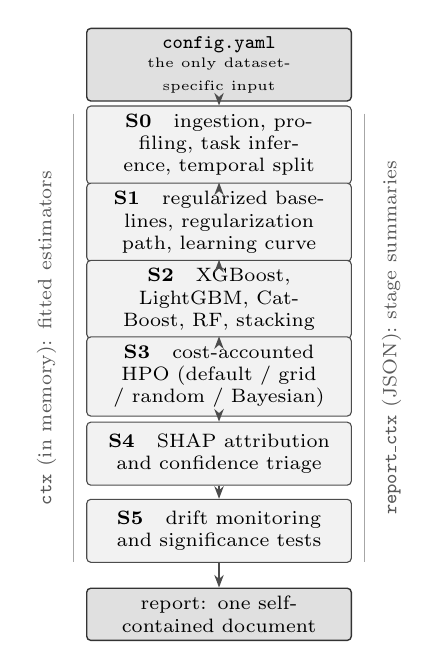
\begin{tikzpicture}[
  font=\scriptsize,
  stage/.style={draw=black!70, fill=black!5, rounded corners=1.5pt,
                text width=3.15cm, minimum height=0.80cm, align=center,
                inner sep=3pt, line width=0.4pt},
  io/.style={draw=black!80, fill=black!12, rounded corners=1.5pt,
             text width=3.15cm, minimum height=0.56cm, align=center,
             inner sep=3pt, line width=0.5pt},
  ar/.style={-{Stealth[length=1.6mm]}, line width=0.5pt, black!70}
]
\node[io] (cfg) at (0,0) {\texttt{config.yaml}\\[-1pt]\textnormal{\tiny the only dataset-specific input}};
\node[stage] (s0) at (0,-1.02) {\textbf{S0}\quad ingestion, profiling, task inference, temporal split};
\node[stage] (s1) at (0,-2.00) {\textbf{S1}\quad regularized baselines, regularization path, learning curve};
\node[stage] (s2) at (0,-2.98) {\textbf{S2}\quad XGBoost, LightGBM, CatBoost, RF, stacking};
\node[stage] (s3) at (0,-3.96) {\textbf{S3}\quad cost-accounted HPO (default / grid / random / Bayesian)};
\node[stage] (s4) at (0,-4.94) {\textbf{S4}\quad SHAP attribution and confidence triage};
\node[stage] (s5) at (0,-5.92) {\textbf{S5}\quad drift monitoring and significance tests};
\node[io] (rep) at (0,-6.98) {report: one self-contained document};

\draw[ar] (cfg) -- (s0);
\draw[ar] (s0) -- (s1);
\draw[ar] (s1) -- (s2);
\draw[ar] (s2) -- (s3);
\draw[ar] (s3) -- (s4);
\draw[ar] (s4) -- (s5);
\draw[ar] (s5) -- (rep);

% two cross-cutting data objects threaded through every stage
\draw[black!35, line width=0.4pt] (-1.85,-0.62) -- (-1.85,-6.32);
\draw[black!35, line width=0.4pt] (1.85,-0.62) -- (1.85,-6.32);
\node[rotate=90, font=\scriptsize, text=black!65, anchor=center]
  at (-2.19,-3.47) {\texttt{ctx} \textnormal{(in memory): fitted estimators}};
\node[rotate=90, font=\scriptsize, text=black!65, anchor=center]
  at (2.19,-3.47) {\texttt{report\_ctx} \textnormal{(JSON): stage summaries}};
\end{tikzpicture}
\caption{Stage graph of the TabML-Guard pipeline. The configuration file is the only dataset-specific input. Every stage reads and writes the in-memory context \texttt{ctx}; only the JSON-serializable \texttt{report\_ctx} survives to the final report, which is assembled from it alone.}
\label{fig:arch}
\end{figure}

\subsection{Stage S0: Ingestion, profiling, and the temporal split}
The loader supports OpenML datasets by numeric identifier or by name and version, and local CSV files. Profiling records the shape, per-column dtypes, total and per-column missingness, the target's class balance or summary statistics, and the time span. Task inference is a heuristic over the target column: a text, boolean, or low-cardinality integer target indicates classification, and a continuous numeric target indicates regression. The inference is overridable, but in our experiments it was correct on all three datasets without intervention. A categorical feature with more than fifty distinct values raises a warning, because dense one-hot encoding of such a column is usually a sign that an identifier should have been dropped.

The split is temporal. Rows are sorted by the time column with a stable mergesort and cut once at the configured fraction, with the earliest rows forming the training set and the latest forming the test set. When no time column is supplied the pipeline falls back to a random split and skips the drift stage, since drift is not identifiable from a shuffled sample. Preprocessing is a column transformer that median-imputes and standardizes numeric columns and most-frequent-imputes and one-hot-encodes categorical ones.

This design choice is the one that most affects every number that follows. A random split on time-ordered data allows the model to interpolate between temporally adjacent training rows, which inflates the measured score and hides exactly the phenomenon that determines whether the model is useful: decay under distribution shift. Section~\ref{sec:results} shows the material consequence: the same dataset that looks stationary under a temporal split exhibits mean PSI values an order of magnitude beyond the ``large shift'' threshold.

\subsection{Stage S1: Regularized baselines and the regularization path}
The baseline layer fits four linear models at a common regularization strength: no penalty, $L_2$, $L_1$, and elastic net. For classification these are logistic regressions under the corresponding penalties, and for regression they are ordinary least squares, Ridge, Lasso, and elastic net. Formally, the elastic-net objective for a linear predictor with weights $w$ and intercept $b$ is

\begin{equation}
\min_{w,b}\ \frac{1}{2n}\sum_{i=1}^{n}\bigl(y_i - w^{\top}x_i - b\bigr)^2
+ \lambda\Bigl(\alpha\lVert w\rVert_1 + \tfrac{1-\alpha}{2}\lVert w\rVert_2^2\Bigr),
\label{eq:enet}
\end{equation}

where $\alpha \in [0,1]$ interpolates between the lasso ($\alpha=1$) and ridge ($\alpha=0$) and $\lambda \ge 0$ controls overall shrinkage. Larger $\lambda$ shrinks the $L_2$ norm of $w$ smoothly and, under the $L_1$ term, drives individual coefficients exactly to zero.

The baseline layer reports three diagnostics beyond the metrics. Coefficient diagnostics report the fraction of coefficients driven to zero, the $L_1$ and $L_2$ norms, and the strongest features. A regularization path sweeps $\lambda$ over twelve logarithmically spaced values and records, at each strength, how many coefficients survive, the $L_2$ norm, and a validation score. The path is fitted on an internal split of the training data only. A learning curve on the best baseline, using time-series cross-validation when a time column exists, exposes the bias--variance position. These diagnostics exist because the metrics alone can be uninformative, as they were on our primary dataset, where all four penalties produced the same score to five decimal places. The path makes the mechanism visible even when the endpoint is flat.

\subsection{Stage S2: Boosting ensembles and stacking}
The ensemble layer fits XGBoost \cite{chen2016xgboost}, LightGBM \cite{ke2017lightgbm}, CatBoost \cite{prokhorenkova2018catboost}, and a random forest \cite{breiman2001random} as a non-boosted reference, followed by a stacked generalization \cite{wolpert1992stacked} whose meta-learner is a regularized linear model. All base learners share a fixed default configuration (three hundred trees, learning rate $0.1$, depth six, subsampling at $0.9$) so that Stage S3 has a meaningful ``untuned'' point of comparison. Each booster is constructed by a builder that imports its library lazily; an absent library causes that model to be skipped with a recorded note.

Gradient boosting builds an additive model $F_M(x)=\sum_{m=1}^{M}\gamma_m h_m(x)$ of weak learners $h_m$, fitting each new tree to the negative gradient of the loss at the current prediction \cite{friedman2001greedy}:

\begin{equation}
h_m = \arg\min_{h}\ \sum_{i=1}^{n}\Bigl[-\frac{\partial L(y_i, F(x_i))}{\partial F(x_i)}\bigg|_{F=F_{m-1}} - h(x_i)\Bigr]^2.
\label{eq:gbm}
\end{equation}

Stacking poses one implementation subtlety that is worth recording because it is a common source of silent leakage. Scikit-learn's stacking implementation builds meta-features with out-of-fold predictions, which requires the cross-validation splitter to be a partition, with every row appearing in exactly one validation fold. A forward-chaining time-series splitter is not a partition, since its earliest rows are never validated, and it raises. Stacking therefore uses stratified or plain $k$-fold internally. Temporal honesty is preserved because the held-out temporal test set is not part of that inner cross-validation; it is scored only once, at the end. Hyperparameter search, by contrast, scores folds with a different scikit-learn entry point that tolerates a non-partition splitter and can therefore use the time-series splitter directly. Both behaviours are correct, and the distinction between them is the kind of thing that is easy to get wrong and hard to notice.

\subsection{Stage S3: Cost-accounted hyperparameter optimization}
The strongest booster from Stage S2 is tuned four ways at a matched budget. \emph{Default} uses the Stage S2 configuration unchanged and serves as the reference. \emph{Grid} search enumerates a coarse discrete lattice. \emph{Random} search samples the same continuous ranges uniformly for exactly $T$ candidates. \emph{Bayesian} search uses Optuna's tree-structured Parzen estimator \cite{akiba2019optuna} for the same $T$ candidates. Because random and Bayesian receive identical candidate budgets and identical cross-validation splits, the head-to-head between them isolates the value of the surrogate model.

Each hyperparameter is declared once and consumed three ways (as a discrete grid, as a continuous range for the sampler, and as a suggestion call for the surrogate), so all strategies explore the same region of the same space and only the search policy varies. For each strategy the pipeline records the best configuration, the cross-validated score, the number of candidate configurations, the number of model evaluations (candidates times folds), and the wall-clock seconds.

Two details keep the comparison fair. First, searches run without refitting; the winning configuration is read from the search results and then refit exactly once through the same evaluation path as every other model, so its leaderboard row is directly comparable to Stages S1 and S2 and is scored on data the search never saw. Second, all Stage S3 fits use a fixed, modest tree budget and are pinned to a single thread, so that outer parallelism over candidates or folds owns the cores and the machine is not oversubscribed by a factor of the core count squared.

The stage emits a verdict expressed as the gain over the untuned default together with the cost that produced it, and it promotes a tuned model to champion status only if it leads on the held-out test set. Formally we report the cost-normalized return

\begin{equation}
R(\theta) = \frac{M(\theta_{\text{default}}) - M(\theta_{\text{tuned}})}{M(\theta_{\text{default}})} \Big/ C(\theta),
\label{eq:return}
\end{equation}

where $M$ is the held-out metric oriented so that higher is better, $\theta$ denotes the configuration, and $C$ is the wall-clock cost of the search that produced it. $R$ is the quantity a practitioner actually needs and the quantity a leaderboard omits.

\subsection{Stage S4: SHAP explanation and reliability triage}
The champion model is explained with SHAP \cite{lundberg2017unified}. Shapley values assign to feature $j$ of instance $x$ its average marginal contribution over all feature subsets:

\begin{equation}
\phi_j(x) = \sum_{S \subseteq N \setminus \{j\}} \frac{|S|!\,(|N|-|S|-1)!}{|N|!}\bigl[f(S \cup \{j\}) - f(S)\bigr],
\label{eq:shap}
\end{equation}

where $N$ is the full feature set and $f(S)$ is the model's output restricted to $S$. Attributions are additive, so $\sum_j \phi_j(x) = f(x) - \mathbb{E}[f]$.

The explainer is chosen by model type: a tree explainer for models exposing feature importances, a linear explainer for models exposing coefficients, and a model-agnostic fallback otherwise. This routing matters more than it might appear. On our primary classification dataset the champion was a regularized linear model rather than a tree ensemble, so a pipeline hard-wired to a tree explainer would have failed on its own headline case. Attributions are computed in the transformed feature space in which the model operates and relabelled with the preprocessing transformer's output feature names, so that importances align with real columns rather than encoded ones.

The reliability layer is independent of SHAP and uses only the probabilities the model already produces. Let $c(x) = \max_k p_k(x)$ be the predicted confidence. Predictions are ranked by confidence and the least-confident fraction $q$ is routed to human review. The layer reports three quantities: the flagged coverage $q$; the \emph{error-capture rate}, defined as the fraction of all errors that fall in the flagged slice,

\begin{equation}
\mathrm{ECR}(q) = \frac{\bigl|\{i : \hat{y}_i \ne y_i \ \wedge\ c(x_i) \le \tau_q\}\bigr|}{\bigl|\{i : \hat{y}_i \ne y_i\}\bigr|},
\label{eq:ecr}
\end{equation}

where $\tau_q$ is the $q$-quantile of confidence; and the accuracy of the auto-accepted remainder against the accuracy of the flagged slice. It also bins accuracy by confidence to produce a calibration-style reliability curve. A routing rule is only worth deploying if $\mathrm{ECR}(q) \gg q$; the results in Section~\ref{sec:results} report whether that held.

\subsection{Stage S5: Drift monitoring and significance testing}
The temporal test set is cut into $n$ consecutive chunks. A frozen model, trained once on the training period, is scored on each chunk in turn, a walk-forward, prequential evaluation \cite{gama2014survey}. In parallel an adaptive model predicts each chunk \emph{before} being retrained on it, under one of three policies: no retraining, periodic retraining over an expanding window, or sliding-window retraining over a fixed recent horizon. The adaptive model clones the entire pipeline at each refit, so imputation and scaling statistics are relearned on the new window rather than inherited from the original fit. The absence of look-ahead is structural: the prediction for chunk $i$ is made before chunk $i$ is observed by the learner.

Covariate shift is tracked per feature against the training distribution using the Population Stability Index,

\begin{equation}
\mathrm{PSI} = \sum_{b=1}^{B}\bigl(p_b^{\text{ref}} - p_b^{\text{cur}}\bigr)\ln\!\frac{p_b^{\text{ref}}}{p_b^{\text{cur}}},
\label{eq:psi}
\end{equation}

where $p_b^{\text{ref}}$ and $p_b^{\text{cur}}$ are the proportions of observations falling in bin $b$ of the reference and current windows respectively. We follow the credit-scoring convention that values above $0.1$ indicate a moderate shift and above $0.2$ a large one \cite{siddiqi2005credit}. An optional adaptive-windowing change detector \cite{bifet2007adwin} runs over the frozen model's error stream as a second signal.

Every comparative claim is tested. For two classifiers evaluated on the same held-out rows, the relevant disagreement is confined to the rows on which they differ. Let $n_{01}$ count the rows where the first model errs and the second is correct, and $n_{10}$ the converse. McNemar's test \cite{mcnemar1947note} evaluates

\begin{equation}
\chi^2 = \frac{(|n_{01} - n_{10}| - 1)^2}{n_{01} + n_{10}},
\label{eq:mcnemar}
\end{equation}

with a continuity correction, falling back to an exact binomial test when the number of discordant rows is small; the null hypothesis is that the two models are equally likely to be correct on the rows where they disagree. For regression, where no such paired correctness notion exists, we apply the Wilcoxon signed-rank test \cite{wilcoxon1945individual} to the paired absolute errors. Three comparisons are adjudicated automatically: champion against runner-up, champion against the simplest linear baseline, and frozen against adaptive.

\subsection{Report generation}
The final stage renders everything into one document: a verdict panel naming the recommended model and its primary score, the headline finding, then per-stage sections with the diagnostics, and finally a reproducibility footer carrying the configuration, library versions, and random seed. Figures are embedded as base64 payloads so the file is portable, and the Stage S1 regularization-path plots are drawn as inline vector graphics rather than raster images. The document is written for a reader who will make a decision from it rather than one who will re-run it.

\section{Experimental Design}
\label{sec:experiments}

\subsection{Datasets}
We chose three datasets that differ in task type, size, dimensionality, and signal-to-noise ratio, so that any conclusion that holds across all three is not an artifact of one regime. Table~\ref{tab:datasets} summarizes them.

\textbf{D1: ELEC2 electricity price movement} \cite{drift2024}. Half-hourly records of the Australian New South Wales electricity market, with the binary target indicating whether the price rises or falls relative to a moving average. It is the standard benchmark in the concept-drift literature and the dataset used by the drift paper that motivated this work. It is time-ordered, binary, mildly imbalanced, and small enough in feature count that a linear model is a serious contender.

\textbf{D2: Appliances energy consumption.} Ten-minute observations of a low-energy house, with the target being appliance energy use in watt-hours. Twenty-seven numeric features describe indoor and outdoor temperature and humidity, pressure, wind speed, and visibility. The target is heavy-tailed and the features are dominated by diurnal and seasonal structure.

\textbf{D3: Metro interstate traffic volume.} Hourly traffic volume on a Minnesota interstate with weather covariates, spanning six years. It has the largest row count, the coarsest target granularity, and the strongest weekly and annual seasonality of the three.

\begin{table}[t]
\caption{Summary of the three evaluation datasets. Missingness for D3 is confined to a single holiday column that is almost entirely absent.}
\label{tab:datasets}
\centering
\footnotesize
\setlength{\tabcolsep}{3pt}
\begin{tabular}{lccc}
\toprule
Property & D1 ELEC2 & D2 Appliances & D3 Metro \\
\midrule
Task & Classification & Regression & Regression \\
Rows & 45{,}312 & 19{,}735 & 48{,}204 \\
Features used & 7 & 27 & 7 \\
Target balance & 57.6 / 42.4 & --- & --- \\
Target range & $\{$UP, DOWN$\}$ & 10--1080 & 0--7280 \\
Target mean (SD) & --- & 97.7 (102.5) & 3259.8 (1986.9) \\
Train / test rows & 27{,}187 / 18{,}125 & 11{,}841 / 7{,}894 & 28{,}922 / 19{,}282 \\
Time span & 1996--1998 & Jan--May 2016 & 2012--2018 \\
\bottomrule
\end{tabular}
\end{table}

\subsection{Configuration}
All three runs used an identical configuration apart from dataset-specific fields: a $60/40$ temporal split, the four boosters plus stacking, a tuning budget of $T=40$ candidate configurations with three time-series cross-validation folds, ten drift chunks, and sliding-window retraining. The random seed was fixed at $42$ for every splitter, model, and sampler. The only per-dataset deviations were the data source, target column, time column, and, for D3, dropping a holiday column that was missing in $99.9\%$ of rows.

\subsection{Metrics}
Classification runs report accuracy, precision, recall, $F_1$, $F_2$ (with $\beta = 2$, weighting recall above precision), ROC-AUC, and PR-AUC. Regression runs report mean absolute error (MAE), root-mean-square error (RMSE), and the coefficient of determination ($R^2$). Model selection within a run used ROC-AUC for classification and negative RMSE for regression, in both cases on the cross-validated training folds; all reported scores are computed once on the temporally held-out test set.

The choice of $F_2$ alongside ROC-AUC is deliberate. The two encode different operational costs of error, and Section~\ref{sec:results} shows that they select different champions on the same dataset, which is the practical form of the observation that metric choice is a modelling decision rather than a reporting detail.

\subsection{Implementation and reproducibility}
The pipeline is implemented in Python against scikit-learn, XGBoost, LightGBM, CatBoost, Optuna, SHAP, statsmodels, and \texttt{river}, pinned by a requirements file with minimum versions. Stage S3 pins base learners to a single thread while parallelizing the outer search, so that the wall-clock costs reported in Section~\ref{sec:results} are not distorted by oversubscription. Reported timings are single-machine wall-clock measurements and are therefore indicative rather than portable; we treat the \emph{ratios} between strategies as the transferable quantity.

\section{Results}
\label{sec:results}

\subsection{Regularization strength was almost inert}
Table~\ref{tab:baselines} reports the four regularized baselines on each dataset. On D1 the four penalties, including no penalty at all, produced ROC-AUC values within $2.0\times10^{-5}$ of one another. On D2 the entire span across the four regularizers was $0.23$ RMSE, or $0.24\%$ of the metric; on D3 it was $0.94$ RMSE, or $0.05\%$.

\begin{table}[t]
\caption{Stage S1 regularized baselines on the temporally held-out test set. The spread column gives the range between the best and worst regularizer.}
\label{tab:baselines}
\centering
\footnotesize
\setlength{\tabcolsep}{3pt}
\begin{tabular}{llccc}
\toprule
Dataset & Baseline & Primary metric & Value & Fit (s) \\
\midrule
\multirow{4}{*}{D1} & No penalty & ROC-AUC & 0.78841 & 0.08 \\
 & $L_2$ (ridge) & ROC-AUC & 0.78842 & 0.07 \\
 & $L_1$ (lasso) & ROC-AUC & \textbf{0.78843} & 0.50 \\
 & Elastic net & ROC-AUC & 0.78842 & 0.47 \\
 & \multicolumn{2}{l}{\emph{spread}} & $2.0\times10^{-5}$ & \\
\midrule
\multirow{4}{*}{D2} & Linear (OLS) & RMSE & \textbf{94.12} & 0.05 \\
 & $L_2$ (ridge) & RMSE & 94.16 & 0.03 \\
 & $L_1$ (lasso) & RMSE & 94.13 & 19.42 \\
 & Elastic net & RMSE & 94.35 & 14.05 \\
 & \multicolumn{2}{l}{\emph{spread}} & 0.23 & \\
\midrule
\multirow{4}{*}{D3} & Linear (OLS) & RMSE & 1922.19 & 0.18 \\
 & $L_2$ (ridge) & RMSE & 1921.92 & 0.06 \\
 & $L_1$ (lasso) & RMSE & 1922.47 & 130.45 \\
 & Elastic net & RMSE & \textbf{1921.53} & 19.71 \\
 & \multicolumn{2}{l}{\emph{spread}} & 0.94 & \\
\bottomrule
\end{tabular}
\end{table}

This flatness is not a failure of regularization. When the number of rows greatly exceeds the number of features, the empirical risk minimizer is already well determined; the penalty term, at a strength chosen by cross-validation, is a small perturbation on an objective that is not ill-posed. The mechanism is nonetheless real, and the regularization path makes it visible. On D1, sweeping the inverse regularization strength over eight orders of magnitude shows the $L_1$ path retaining only $2$ of $13$ encoded features at the strongest penalty and rising to all $13$ as the penalty relaxes, while the $L_2$ path shrinks the coefficient norm monotonically and never zeroes a coefficient. On D2 the lasso path retains $5$ of $27$ features at its strongest setting; on D3 it retains $10$ of $61$. So the regularization mechanism operates as theory predicts; it simply does not move the held-out score when the data are plentiful relative to the feature count.

There is a second, practical lesson in Table~\ref{tab:baselines}. The $L_1$ fits cost two to three orders of magnitude more time than the $L_2$ or unpenalized fits ($130$ seconds against $0.06$ seconds on D3), because the coordinate-descent solver converges slowly at the scale of these feature counts. That is a real cost paid for a score difference in the fourth decimal place.

\subsection{No model family won universally}
Table~\ref{tab:leaderboard} reports the best model of each family per dataset. The pattern is mixed, and it does not support the reflexive preference for boosting.

On D1, the best model overall was the $L_1$-penalized logistic regression at ROC-AUC $0.7884$, ahead of CatBoost at $0.7814$, LightGBM at $0.7742$, XGBoost at $0.7739$, the stacked ensemble at $0.7730$, and the random forest at $0.7718$. On D2 the linear model won by a wide margin: the ordinary least squares fit reached RMSE $94.12$ while every boosting model was worse than predicting the mean, with CatBoost at $118.60$ ($R^2 = -0.49$), LightGBM at $147.03$, and XGBoost at $222.70$ ($R^2 = -4.24$). Only on D3 did a booster win, with CatBoost at RMSE $1894.39$ against the elastic-net baseline's $1921.53$ ($R^2 = 0.081$ versus $0.054$).

\begin{table}[t]
\caption{Best model per family on the temporally held-out test set. The champion row for each dataset is shown in bold. ``Fit'' is the single-fit wall-clock time in seconds.}
\label{tab:leaderboard}
\centering
\footnotesize
\setlength{\tabcolsep}{3pt}
\begin{tabular}{llccc}
\toprule
Dataset & Model & Primary & $R^2$/Acc. & Fit (s) \\
\midrule
\multirow{6}{*}{D1} & \textbf{Logistic ($L_1$)} & \textbf{0.7884} & 0.7246 & 0.50 \\
 & CatBoost & 0.7814 & 0.7105 & 3.13 \\
 & LightGBM & 0.7742 & 0.7007 & 0.67 \\
 & XGBoost & 0.7739 & 0.7001 & 0.86 \\
 & Stacking & 0.7730 & 0.7049 & 29.07 \\
 & Random forest & 0.7718 & 0.7085 & 1.26 \\
\midrule
\multirow{6}{*}{D2} & \textbf{Linear (OLS)} & \textbf{94.12} & 0.065 & 0.05 \\
 & CatBoost & 118.60 & $-0.485$ & 1.10 \\
 & LightGBM & 147.03 & $-1.282$ & 0.26 \\
 & Random forest & 163.02 & $-1.806$ & 4.05 \\
 & Stacking & 198.97 & $-3.180$ & 17.91 \\
 & XGBoost & 222.70 & $-4.236$ & 0.54 \\
\midrule
\multirow{5}{*}{D3} & \textbf{CatBoost} & \textbf{1894.39} & 0.081 & 1.12 \\
 & LightGBM & 1909.61 & 0.066 & 0.30 \\
 & Stacking & 1911.96 & 0.064 & 12.84 \\
 & XGBoost & 1921.51 & 0.054 & 0.50 \\
 & Random forest & 2181.71 & $-0.219$ & 2.10 \\
\bottomrule
\end{tabular}
\end{table}

The D2 result deserves comment because it is the strongest evidence against the boilerplate workflow. The boosting models were not merely marginally worse; they were far below a model that predicts the training mean. A gradient-boosted tree with three hundred rounds and a learning rate of $0.1$ will fit the training distribution closely, and when the signal is weak and the target is heavy-tailed, that fit is noise. The default configuration that makes boosting models strong on large datasets makes them actively harmful on small, noisy ones. A pipeline that always tunes its booster, as AutoML systems do, would spend its budget optimizing within a family that should not have been selected at all.

Finally, the stacking meta-model never won. It was competitive on D1 ($0.7730$, mid-pack) and on D3 ($1911.96$, third of nine), and it was the second-worst model on D2. It was also, consistently, the most expensive model to fit: $29$ seconds on D1 against $0.5$ seconds for the linear champion, because it cross-validates every base learner to build meta-features. The regularized stacking idea \cite{regstack2025} is sound in principle, but on these datasets it did not buy back its cost.

\subsection{Metric choice moved the winner}
On D1 the ranking by ROC-AUC and the ranking by $F_2$ disagree, and the disagreement is large. The linear champion has the best ROC-AUC ($0.7884$) but the worst $F_2$ of the six candidates ($0.5667$), because it is conservative: recall of $0.535$ against precision of $0.743$. XGBoost has a lower ROC-AUC ($0.7739$) but the best $F_2$ by a clear margin ($0.6712$), on recall of $0.680$ and precision of $0.637$. If the operational cost of a missed positive is the dominant concern, which is what $\beta = 2$ encodes, the correct choice on this dataset is the model that ROC-AUC ranks fourth.

The pipeline reports both, and neither is privileged. But the result is a reminder that a single headline metric is a modelling decision, and that comparing systems by whichever metric they chose to report is not a comparison at all.

\subsection{Tuning's return ranged from substantial to negative}
This is the paper's central result. Table~\ref{tab:tuning} reports the four strategies on three datasets with the wall-clock cost and the resulting held-out score, and Fig.~\ref{fig:cost} shows the same data as a cost--benefit plane.

\begin{table}[t]
\caption{Stage S3 hyperparameter-optimization strategies. Wall-clock is the search cost in seconds; evaluations is candidates times cross-validation folds. The final column is the relative change in the held-out metric against the untuned default.}
\label{tab:tuning}
\centering
\footnotesize
\setlength{\tabcolsep}{3pt}
\begin{tabular}{llccc}
\toprule
Dataset & Strategy & Wall (s) & Evals & $\Delta$ vs default \\
\midrule
\multirow{4}{*}{D1} & Default & 2.6 & 1 & --- \\
 & Grid & 11.2 & 54 & $+0.38\%$ \\
 & Random & 48.9 & 120 & $+0.56\%$ \\
 & Bayesian & 149.1 & 120 & $+0.59\%$ \\
\midrule
\multirow{4}{*}{D2} & Default & 2.8 & 1 & --- \\
 & Grid & 22.8 & 54 & $+12.63\%$ \\
 & Random & 193.9 & 120 & $+15.15\%$ \\
 & Bayesian & 838.5 & 120 & $+18.24\%$ \\
\midrule
\multirow{4}{*}{D3} & Default & 1.2 & 1 & --- \\
 & Grid & 9.0 & 54 & $-0.62\%$ \\
 & Random & 24.4 & 120 & $-0.40\%$ \\
 & Bayesian & 72.3 & 120 & $-0.66\%$ \\
\bottomrule
\end{tabular}
\end{table}

\begin{figure}[t]
\centering
\begin{tikzpicture}
\begin{axis}[
  width=\columnwidth, height=4.4cm,
  xmode=log,
  xlabel={Hyperparameter-search wall-clock cost (s, log scale)},
  ylabel={Gain over untuned default (\%)},
  xlabel style={font=\scriptsize},
  ylabel style={font=\scriptsize},
  tick label style={font=\scriptsize, color=black!60},
  grid=major,
  grid style={draw=black!12, line width=0.3pt},
  axis line style={draw=black!45, line width=0.4pt},
  tick align=outside,
  ymin=-3.4, ymax=22.5, xmin=0.9, xmax=2600,
  legend style={font=\scriptsize, draw=none, fill=none,
                at={(0.015,0.985)}, anchor=north west},
  legend cell align=left,
]
% zero line: below it, tuning made the model worse than not tuning
\addplot[black!35, line width=0.5pt, forget plot]
  coordinates {(0.9,0) (2600,0)};

% ---- D1: ELEC2, ROC-AUC (higher better) ----
\addplot[dOne, line width=0.9pt, forget plot]
  coordinates {(2.64,0) (11.22,0.381) (48.94,0.557) (149.13,0.590)};
\addlegendentry{D1 ELEC2 (ROC-AUC)}
\addplot[dOne, only marks, mark=*, mark size=1.6pt, forget plot] coordinates {(2.64,0)};
\addplot[dOne, only marks, mark=square*, mark size=1.6pt, forget plot] coordinates {(11.22,0.381)};
\addplot[dOne, only marks, mark=triangle*, mark size=1.9pt, forget plot] coordinates {(48.94,0.557)};
\addplot[dOne, only marks, mark=diamond*, mark size=1.9pt, forget plot] coordinates {(149.13,0.590)};

% ---- D2: Appliances, RMSE (lower better) ----
\addplot[dTwo, line width=0.9pt, forget plot]
  coordinates {(2.82,0) (22.79,12.63) (193.87,15.15) (838.45,18.24)};
\addlegendentry{D2 Appliances (RMSE)}
\addplot[dTwo, only marks, mark=*, mark size=1.6pt, forget plot] coordinates {(2.82,0)};
\addplot[dTwo, only marks, mark=square*, mark size=1.6pt, forget plot] coordinates {(22.79,12.63)};
\addplot[dTwo, only marks, mark=triangle*, mark size=1.9pt, forget plot] coordinates {(193.87,15.15)};
\addplot[dTwo, only marks, mark=diamond*, mark size=1.9pt, forget plot] coordinates {(838.45,18.24)};

% ---- D3: Metro traffic, RMSE (lower better) ----
\addplot[dThree, line width=0.9pt, forget plot]
  coordinates {(1.22,0) (8.99,-0.616) (24.44,-0.400) (72.25,-0.657)};
\addlegendentry{D3 Metro traffic (RMSE)}
\addplot[dThree, only marks, mark=*, mark size=1.6pt, forget plot] coordinates {(1.22,0)};
\addplot[dThree, only marks, mark=square*, mark size=1.6pt, forget plot] coordinates {(8.99,-0.616)};
\addplot[dThree, only marks, mark=triangle*, mark size=1.9pt, forget plot] coordinates {(24.44,-0.400)};
\addplot[dThree, only marks, mark=diamond*, mark size=1.9pt, forget plot] coordinates {(72.25,-0.657)};

% endpoint labels: the gain each dataset's tuning actually bought
\node[font=\scriptsize, color=black!70, anchor=west]
  at (axis cs:190,8.5) {D2 $+18.2\%$};
\node[font=\scriptsize, color=black!70, anchor=west]
  at (axis cs:190,1.9) {D1 $+0.6\%$};
\node[font=\scriptsize, color=black!70, anchor=west]
  at (axis cs:95,-2.3) {D3 $-0.7\%$};
\end{axis}
\end{tikzpicture}
\caption{Hyperparameter search as a cost--benefit problem. Each curve is one dataset; marker shape encodes the search strategy, from circle for the untuned default through square for grid and triangle for random to diamond for Bayesian. The vertical axis is the change in the held-out test metric against the untuned default, oriented so that higher is always better, and the horizontal axis is the wall-clock cost of the search on a logarithmic scale. The zero line is the decision boundary: points below it are strategies that left the model worse than not tuning at all.}
\label{fig:cost}
\end{figure}

Three observations follow.

\textbf{The return on tuning is dataset-dependent to the point of changing sign.} On D2, tuning was unambiguously worthwhile: Bayesian search cut held-out RMSE by $18.2\%$, from $118.60$ to $96.97$. On D1 the entire four-strategy range spanned $0.0046$ ROC-AUC, or $0.59\%$, and the tuned model still finished below the untuned linear baseline. On D3 every strategy made the model worse, by between $0.40\%$ and $0.66\%$. A workflow that tunes by default, as most automated pipelines do, would have spent its budget improving the model on one of three datasets and degrading it on another.

\textbf{The cost of that return is super-linear.} Grid search is the cheapest strategy that explores more than a single point, because it evaluates a fixed coarse lattice. Random and Bayesian search were given identical budgets of $40$ candidates, or $120$ evaluations with three folds. At that matched budget, Bayesian search beat random search on two of three datasets (D1: $0.7860$ against $0.7858$; D2: RMSE $96.97$ against $100.63$) and lost on the third (D3: $1906.85$ against $1901.96$). The margins on D1 are negligible; the margin on D2 is meaningful. But Bayesian search cost $3.1$ times random search on D1 ($149.1$ s against $48.9$ s), $4.3$ times on D2 ($838.5$ s against $193.9$ s), and $3.0$ times on D3 ($72.3$ s against $24.4$ s). Applied to Eq.~\eqref{eq:return}, the surrogate model was repaid on D2 and was not repaid on D1 or D3.

\textbf{Grid search's lattice was too coarse to matter.} On all three datasets grid search returned the same learning rate ($0.03$) and the same $L_2$ leaf regularization ($5.0$), the corner of the lattice on those two axes, and varied the depth only between $4$ and $8$. On D2, where a deeper model was better, grid search reached depth $8$ while both random and Bayesian search reached depth $10$, and Bayesian search's deeper configuration was the best of the twelve candidates evaluated across the three datasets. The grid could not express the optimum that the continuous searches found, and it also never moved on the two axes where a corner solution is least likely to be optimal. This is the argument for random and sequential search in miniature, and it is also why grid search's apparent cheapness is partly an artifact of its low resolution rather than of its efficiency.

The tuned models need one more piece of context. Even after $18.2\%$ of improvement on D2, the tuned CatBoost model reached RMSE $96.97$, still worse than the untuned ordinary least squares fit at $94.12$. And on D1, the most expensive search in the study produced ROC-AUC $0.7860$, below the untuned linear champion's $0.7884$. In two of three cases, the correct conclusion was that the ensemble should not have been tuned, and arguably should not have been chosen.

\subsection{Triage works, and its yield is measurable}
On D1, flagging the least-confident 20\% of test predictions captured 34.2\% of all errors (1706 of 4991). The auto-accepted 80\% was 77.3\% accurate, against 52.9\% on the flagged slice, a separation of 24.4 percentage points. Fig.~\ref{fig:reliability} shows the underlying reliability curve.

\begin{figure}[t]
\centering
\includegraphics[width=\columnwidth]{d1_reliability.png}
\caption{Reliability of the D1 champion. Accuracy is binned by the model's own predicted confidence. The monotone rise is the property that makes confidence-based triage viable: the model's stated certainty tracks its empirical correctness.}
\label{fig:reliability}
\end{figure}

The curve is close to monotone across ten confidence deciles, rising from 50.7\% accuracy in the lowest decile (mean confidence $0.561$) to 94.8\% in the highest (mean confidence $0.985$), with one small inversion between deciles six and seven. Monotonicity is the entire precondition for the routing rule to be rational: if confidence did not track correctness, ranking by it would select an arbitrary subset. Here it does, and the resulting error-capture ratio of $34.2\%$ against $20\%$ coverage is a factor of $1.7$ of enrichment: modest in absolute terms, but free, requiring neither a second model nor any additional training.

Two qualifications matter. First, the separation is good but not sharp: the flagged slice is still 52.9\% accurate, so routing it to a human means sending over half of it as false alarms. Triage reduces a reviewer's workload by concentrating error, not by isolating it. Second, the D1 champion is a linear model whose confidence is a logistic transform, and it is well calibrated for the structural reason that its loss function is a proper scoring rule. A model with sharper or more poorly calibrated confidence would yield a different curve, and the pipeline reports the curve rather than assuming one.

\subsection{Heavy input drift did not produce performance decay}
All three datasets drifted substantially at the input level. Mean PSI across features peaked at $1.73$ on D1, $5.78$ on D2, and $1.96$ on D3, between nine and twenty-nine times the conventional threshold for a ``large'' shift. Fig.~\ref{fig:drift} and Fig.~\ref{fig:psi} show the performance and PSI trajectories for D1, and the pipeline's adaptive change detector raised $37$ alarms over the ten chunks of that stream.

\begin{figure}[t]
\centering
\includegraphics[width=\columnwidth]{d1_drift_perf.png}
\caption{Walk-forward performance on D1. The frozen model, trained once on the earliest 60\% of rows, is scored on ten consecutive chunks of the held-out period; the adaptive model predicts each chunk before retraining on it.}
\label{fig:drift}
\end{figure}

\begin{figure}[t]
\centering
\includegraphics[width=\columnwidth]{d1_drift_psi.png}
\caption{Population Stability Index on D1 over the same ten chunks, measured against the training window. Values above $0.2$ indicate a large shift; the observed trajectory exceeds that threshold throughout.}
\label{fig:psi}
\end{figure}

Performance did not decay in step with that drift; on all three datasets it improved. On D1 the frozen model's accuracy rose from a mean of $0.658$ over the earliest chunks to $0.829$ over the latest, with no monotone degradation in between; the ten-chunk mean was $0.7247$ for the frozen model and $0.7233$ for the adaptive one, a difference of one part in a thousand. On D2 the frozen model's RMSE fell from $103.23$ early in the stream to $93.45$ late in it, and on D3 from $1922.71$ to $1882.70$. The pipeline's own \emph{worse-over-time} flag was false on every dataset.

This contradicts a naive reading of the drift literature, and the contradiction is only apparent.

The methodological lesson is that covariate shift and concept drift are not the same thing, and PSI measures only the former. A feature can move a long way without the conditional relationship between features and target changing at all. Indeed, when the target is partly a function of the drifting features, as is the case when the model uses temperature to predict traffic, a feature shift can move the model \emph{toward} the region where it was trained more densely. Reporting high PSI as though it implied degraded accuracy would have been wrong here on all three datasets.

Retraining, correspondingly, helped only where the task was regression. On D1 the sliding-window adaptive model did not beat the frozen one (accuracy $0.7233$ against $0.7247$; McNemar $p = 0.398$, not significant). On D2 the adaptive model's MAE was $53.51$ against the frozen model's $59.50$, a difference that is decisively significant ($p = 3.9 \times 10^{-101}$). On D3 the adaptive model's MAE was $1623.44$ against $1635.15$ ($p = 5.0 \times 10^{-18}$). Both regression datasets found retraining worthwhile; the classification dataset did not.

\subsection{Significance testing corrected the leaderboard}
Table~\ref{tab:significance} reports the paired tests. On D1 the top two models on the leaderboard, the $L_1$- and elastic-net-penalized logistic regressions, differed on exactly \emph{one} held-out row out of $18{,}125$. The leaderboard ranked one above the other; McNemar's exact test returned $p = 1.0$. The ranking was noise, and reporting it as a result would have been a mistake.

\begin{table}[t]
\caption{Paired significance tests. McNemar's test for classification, Wilcoxon signed-rank on absolute errors for regression.}
\label{tab:significance}
\centering
\footnotesize
\setlength{\tabcolsep}{3pt}
\begin{tabular}{llcc}
\toprule
Dataset & Comparison & Test & $p$ \\
\midrule
D1 & Champion vs.\ runner-up & McNemar & $1.00$ \\
D1 & Frozen vs.\ adaptive & McNemar & $0.398$ \\
D2 & Linear vs.\ lasso & Wilcoxon & $0.130$ \\
D2 & Frozen vs.\ adaptive & Wilcoxon & $3.9\times10^{-101}$ \\
D3 & Champion vs.\ same-config refit & Wilcoxon & $7.6\times10^{-6}$ \\
D3 & Champion vs.\ linear & Wilcoxon & $9.3\times10^{-28}$ \\
D3 & Frozen vs.\ adaptive & Wilcoxon & $5.0\times10^{-18}$ \\
\bottomrule
\end{tabular}
\end{table}

The D2 baseline comparison shows the same effect in the other direction. The ordinary least squares fit and the lasso differed by $0.039$ in mean absolute error, a difference a leaderboard would report as a ranking, and the Wilcoxon test returned $p = 0.130$, correctly declining to distinguish them. D3 supplies the contrast: a margin of $28.6$ MAE between the CatBoost champion and the elastic-net baseline is highly significant ($p = 9.3 \times 10^{-28}$), because the per-row errors are consistently, not occasionally, better.

D3 also supplies the sharpest caution about what a small $p$-value does and does not mean. The champion-versus-runner-up comparison for that dataset pits \texttt{catboost\_default} against \texttt{catboost}: two fits of the \emph{same} configuration of the \emph{same} model, differing only in the code path that produced them. They differ significantly ($p = 7.6 \times 10^{-6}$). A significant test licenses the claim that the two fits are consistently ordered across these rows; it does not license the claim that either is the better model. Effect size and significance are separate questions, and on a test set of nineteen thousand rows the former can be negligible while the latter is emphatic.

The practical implication is that leaderboard orderings should be treated as hypotheses rather than conclusions. In this study the top two entries were separated by a single row on D1, by a margin a paired test declined to distinguish on D2, and on D3 by a difference between two fits of one configuration.

\subsection{SHAP attributions agreed across model families}
Fig.~\ref{fig:shap} shows global attributions for the champion of each dataset.

\begin{figure}[t]
\centering
\includegraphics[width=\columnwidth]{d1_shap.png}
\caption{Global SHAP attributions for the D1 champion (an $L_1$-penalized logistic regression, explained with the linear explainer). The New South Wales price dominates, followed by demand and interconnector transfer.}
\label{fig:shap}
\end{figure}

On D1 the New South Wales price dominates with a mean absolute attribution of $0.807$, well ahead of New South Wales demand ($0.446$), Victorian demand ($0.413$), and interconnector transfer ($0.399$). This corroborates the model's coefficient structure independently: the same feature led the standardized coefficient ranking. On D3, temperature ($267.5$) leads cloud cover ($187.4$), with the weather category indicators following, a ranking that would be unsurprising to a traffic engineer. On D2, outdoor temperature ($54.3$), dew point ($43.0$), and indoor humidities dominate.

The agreement between SHAP and the coefficient ranking on D1 is not automatic. They are different quantities: a Shapley value is a marginal contribution averaged over subsets, whereas a coefficient is a partial derivative of the linear predictor. They can diverge under correlated features. Their agreement here is mild evidence that the attribution is not an artifact of the explainer. It also illustrates why the explainer routing in Stage S4 matters: on the dataset with the largest sample size the champion was linear, and a tree-only explainer would have had nothing to say about it.

\section{Discussion}
\label{sec:discussion}

\subsection{Why the results look like this}
The three central findings are not independent. Regularization strength was inert, boosting sometimes failed catastrophically, and tuning's return varied in sign. All three follow from the same underlying fact: these datasets are small relative to their noise. D2 has $19{,}735$ rows and a target whose variance is dominated by occupant behaviour that no sensor in the dataset records. In that regime, model capacity is a liability, regularization strength is a minor correction to an already well-determined fit, and hyperparameter search is optimizing a response surface whose curvature is mostly noise.

D3 is the counterexample that shows the mechanism. It has the most rows, the strongest seasonality, and the largest effective feature count after encoding ($61$ features from the categorical weather columns). There, CatBoost beat the linear baseline, and the tuning return, while negative, was negative by a fraction of a percent rather than by a factor. Tuning did not help, but no strategy was actively harmful either: search found nothing better than the default because the default was already near the plateau.

The metric-dependence result fits the same frame. The linear model on D1 has the best ranking metric and the worst $F_2$ because it hedges: its recall is $0.535$, well below the boosters' $\approx 0.68$. When the positive class is the minority and the decision threshold is $\tfrac{1}{2}$, a conservative model wins on a threshold-free ranking metric and loses on a metric that weights the minority class. That is not a defect in either model; it is the ordinary consequence of a dataset whose class balance makes the default threshold a poor operating point.

\subsection{Implications for practice}
\textbf{Do not tune by default.} The instrumentation to decide whether tuning was worth it is cheap (two numbers, a budget and a clock), and the answer changed sign across three datasets in this study. A pipeline that reports only the tuned score hides the case where the search degraded the model.

\textbf{Establish the linear baseline before the ensemble.} On two of three datasets here, the correct model was a regularized linear fit, and on one of them every boosting model was worse than predicting the mean. Fitting four linear models took under two seconds per dataset in total, against $18$ minutes of search to reach a boosting model that still lost.

\textbf{Report the metric that matches the decision.} ROC-AUC and $F_2$ selected different champions on D1. Neither is wrong; publishing one and calling it ``the'' result is.

\textbf{Distinguish covariate shift from concept drift.} PSI exceeded the large-shift threshold on every dataset in this study and measured performance improved on all three rather than decaying. An alarm triggered by PSI alone would have fired constantly and correctly identified nothing.

\textbf{Cheap triage is worth having.} The confidence-based routing rule required no additional model, no retraining, and no extra inference; it concentrated $34\%$ of the errors into $20\%$ of the volume. That is not a decisive gain, but the cost is zero and the operational benefit, letting a reviewer prioritize, is real.

\subsection{Threats to validity}
\textbf{Internal validity.} The pipeline's leakage controls are structural, but our confidence in them rests on design inspection rather than on an adversarial test. A randomized-train/test ablation would quantify the optimism a shuffled split would have introduced; we did not run it, and it is the most obviously missing experiment. Reported wall-clock costs are single-machine measurements and are sensitive to load; we have argued from ratios rather than absolute values, but the ratios were measured once, without repetition or confidence intervals.

\textbf{Construct validity.} PSI is a heuristic with conventional thresholds inherited from credit scoring, and those thresholds were calibrated on a different kind of data. Our use of them is conventional rather than validated. The error-capture rate in Eq.~\eqref{eq:ecr} measures concentration of error but not the value of catching it, which depends on the asymmetry of costs we have not modelled.

\textbf{External validity.} Three datasets is evidence of generality, not proof of it. All three are numeric-dominant, none has more than a few dozen features, and none exceeds fifty thousand rows. The pipeline's behaviour on wide, sparse, high-cardinality tabular data, the regime where one-hot encoding becomes untenable and where CatBoost's native categorical handling is most valuable, is untested here. The D2 result in particular suggests that our conclusions about boosting are conditional on dataset scale, which is exactly what a larger study would test.

\textbf{Conclusion validity.} Every comparison is adjudicated by a paired significance test, which is the main defence here. But the tests are run once per comparison without correction for multiplicity, and the champion-versus-runner-up comparisons are performed on the same data that selected the champion. A properly nested protocol, selecting on an inner split and testing on an outer one, would be stricter, and the significance results reported in Table~\ref{tab:significance} should be read with that caveat.

\subsection{Limitations}
The drift study replays historical time order rather than observing a live stream, so the ``adaptive'' model retrains on data that a real deployment would have received with delay. The reliability layer implements the identification half of explanation-driven error compensation \cite{shapcomp2025}, not its compensation half; it routes predictions to a human rather than correcting them. Explanations use SHAP only, with no LIME and no comparison against alternative attribution methods. The pipeline covers classical and ensemble learning by design and contains no neural models. Finally, the drift paper that motivated the temporal framing uses a continuous-kernel adaptation method we did not implement; our adaptive baseline is a windowed refit, and the comparison is between monitoring policies rather than between adaptation algorithms.

\section{Conclusion}
\label{sec:conclusion}

We presented TabML-Guard, a configuration-driven pipeline that runs the full supervised-learning workflow on time-ordered tabular data and answers four operational questions a leaderboard does not: whether the ensemble earned its complexity, whether tuning paid for its compute, which predictions warrant human review, and whether the model survived its encounter with time. The system is dataset-agnostic by construction: three datasets, two task types, and three feature regimes ran through unchanged code. Its output is a single self-contained report written for the person who owns the decision.

The empirical findings are the substance, and they are largely negative. Regularization strength moved the held-out score by at most $0.24\%$. Boosting ensembles were the best choice on one of three datasets and were catastrophically worse than a linear fit on another. The return on hyperparameter optimization ranged from $+18.2\%$ on the dataset with the weakest signal to $-0.7\%$ on the largest, at a cost that grew super-linearly with the surrogate's sophistication. Input distributions drifted by nine to twenty-nine times the conventional large-shift threshold while measured performance improved rather than decayed. And of three leaderboard ``winners'' over their runner-up, one was separated by a single row out of eighteen thousand.

The obvious extension is an ablation that quantifies the optimism a shuffled split would have introduced on these same datasets. That experiment would turn our structural leakage argument into a measurement. Beyond that, the pipeline's natural growth is toward the regimes it does not yet cover: wide and sparse tabular data where categorical encoding strategy dominates model choice, and a comparative study of adaptation algorithms rather than monitoring policies.

TabML-Guard is released as open source under the MIT license.

\appendices
\section{Declarative search space}
\label{app:space}
Table~\ref{tab:space} shows the search space used in Stage S3 for the CatBoost booster, which won Stage S2 on all three datasets. Each parameter is declared once and consumed three ways (as a grid, as a continuous range, and as a surrogate suggestion), so the three search strategies explore the same region and only the policy varies.

\begin{table}[h]
\caption{Stage S3 search space for CatBoost. The grid column enumerates the lattice used by grid search; the range column bounds the continuous distributions used by random and Bayesian search.}
\label{tab:space}
\centering
\footnotesize
\setlength{\tabcolsep}{3pt}
\begin{tabular}{lcc}
\toprule
Parameter & Grid values & Range \\
\midrule
Depth & $\{4, 6, 8\}$ & $[3, 10]$ (integer) \\
Learning rate & $\{0.03, 0.1, 0.2\}$ & $[10^{-3}, 0.3]$ (log) \\
$L_2$ leaf regularization & $\{1, 3, 5\}$ & $[10^{-2}, 10]$ (log) \\
\midrule
\multicolumn{3}{l}{Grid: $18$ candidates, $54$ evaluations ($3$ folds).} \\
\multicolumn{3}{l}{Random and Bayesian: $40$ candidates, $120$ evaluations each.} \\
\bottomrule
\end{tabular}
\end{table}

\section{Minimal configuration example}
\label{app:config}
Listing~\ref{lst:config} shows the complete configuration that produced the D3 results. Changing the source, target, and time column is the only edit required to run on a different dataset.

\begin{figure}[h]
\footnotesize
\begin{verbatim}
dataset:
  source: csv
  path: data/metro_traffic.csv
  target: traffic_volume
  time_col: date_time
  drop_cols: [holiday]
task: auto
split: {train_frac: 0.6, test_frac: 0.4}
models:
  boosters: [xgboost, lightgbm, catboost,
             random_forest]
  stacking: true
tuning: {budget_trials: 40, cv_splits: 3}
drift: {n_chunks: 10, retrain: sliding}
random_state: 42
\end{verbatim}
\caption{The configuration used for the D3 run. All fields not shown take validated defaults.}
\label{lst:config}
\end{figure}

\section*{Acknowledgment}

The author thanks the maintainers of scikit-learn, XGBoost, LightGBM, CatBoost, Optuna, SHAP, statsmodels, and \texttt{river}, on which this work depends. The ELEC2, Appliances, and Metro Interstate Traffic datasets were obtained from the OpenML and UCI repositories.

\begin{thebibliography}{00}

\bibitem{shwartz2022tabular} R. Shwartz-Ziv and A. Armon, ``Tabular data: Deep learning is not all you need,'' \emph{Inf. Fusion}, vol. 81, pp. 84--90, May 2022.

\bibitem{grinsztajn2022tree} L. Grinsztajn, E. Oyallon, and G. Varoquaux, ``Why do tree-based models still outperform deep learning on typical tabular data?,'' in \emph{Proc. Adv. Neural Inf. Process. Syst. (NeurIPS)}, vol. 35, 2022, pp. 507--520.

\bibitem{sculley2015hidden} D. Sculley \emph{et al.}, ``Hidden technical debt in machine learning systems,'' in \emph{Proc. Adv. Neural Inf. Process. Syst. (NeurIPS)}, vol. 28, 2015, pp. 2503--2511.

\bibitem{paleyes2022challenges} A. Paleyes, R.-G. Urma, and N. D. Lawrence, ``Challenges in deploying machine learning: A survey of case studies,'' \emph{ACM Comput. Surv.}, vol. 55, no. 6, pp. 1--29, Dec. 2022.

\bibitem{feurer2015auto} M. Feurer, A. Klein, K. Eggensperger, J. Springenberg, M. Blum, and F. Hutter, ``Efficient and robust automated machine learning,'' in \emph{Proc. Adv. Neural Inf. Process. Syst. (NeurIPS)}, vol. 28, 2015, pp. 2962--2970.

\bibitem{kotthoff2013auto} L. Kotthoff, C. Thornton, H. H. Hoos, F. Hutter, and K. Leyton-Brown, ``Auto-WEKA: Combined selection and hyperparameter optimization of classification algorithms,'' in \emph{Proc. 19th ACM SIGKDD Int. Conf. Knowl. Discovery Data Mining}, 2013, pp. 847--855.

\bibitem{olson2016tpot} R. S. Olson and J. H. Moore, ``TPOT: A tree-based pipeline optimization tool for automating machine learning,'' in \emph{Proc. Workshop Autom. Mach. Learn.}, 2016, pp. 66--74.

\bibitem{erickson2020autogluon} N. Erickson \emph{et al.}, ``AutoGluon-Tabular: Robust and accurate AutoML for structured data,'' \emph{arXiv:2003.06505}, 2020.

\bibitem{hoerl1970ridge} A. E. Hoerl and R. W. Kennard, ``Ridge regression: Biased estimation for nonorthogonal problems,'' \emph{Technometrics}, vol. 12, no. 1, pp. 55--67, Feb. 1970.

\bibitem{tibshirani1996lasso} R. Tibshirani, ``Regression shrinkage and selection via the lasso,'' \emph{J. Roy. Statist. Soc. B}, vol. 58, no. 1, pp. 267--288, 1996.

\bibitem{zou2005elastic} H. Zou and T. Hastie, ``Regularization and variable selection via the elastic net,'' \emph{J. Roy. Statist. Soc. B}, vol. 67, no. 2, pp. 301--320, Apr. 2005.

\bibitem{wolpert1992stacked} D. H. Wolpert, ``Stacked generalization,'' \emph{Neural Netw.}, vol. 5, no. 2, pp. 241--259, 1992.

\bibitem{regstack2025} H. Rashid, M. Hanzla, T. Berghout, Y. Amirat, A. Banerjee, A. Mamoune, and M. Benbouzid, ``RegStack machine learning model for accurate prediction of tidal stream turbine performance and biofouling,'' \emph{Expert Syst. Appl.}, vol. 283, Art. no. 127766, 2025, doi: 10.1016/j.eswa.2025.127766.

\bibitem{boxgboost2026} X. Zhang, K. Yang, Q. Xiao, and Y. Wang, ``Explainable Bayesian-optimized XGBoost for dual-target batching in copper bath smelting,'' \emph{Expert Syst. Appl.}, vol. 309, Art. no. 131260, 2026, doi: 10.1016/j.eswa.2026.131260.

\bibitem{bergstra2012random} J. Bergstra and Y. Bengio, ``Random search for hyper-parameter optimization,'' \emph{J. Mach. Learn. Res.}, vol. 13, pp. 281--305, Feb. 2012.

\bibitem{snoek2012practical} J. Snoek, H. Larochelle, and R. P. Adams, ``Practical Bayesian optimization of machine learning algorithms,'' in \emph{Proc. Adv. Neural Inf. Process. Syst. (NeurIPS)}, vol. 25, 2012, pp. 2951--2959.

\bibitem{akiba2019optuna} T. Akiba, S. Sano, T. Yanase, T. Ohta, and M. Koyama, ``Optuna: A next-generation hyperparameter optimization framework,'' in \emph{Proc. 25th ACM SIGKDD Int. Conf. Knowl. Discovery Data Mining}, 2019, pp. 2623--2631.

\bibitem{spectral2025} G. Chen, V. Feldmann, and I. Seo, ``On parameter tuning for spectral clustering: Two simple, fast, and effective criteria,'' \emph{IEEE Access}, vol. 13, pp. 1--14, 2025, doi: 10.1109/ACCESS.2025.3623882.

\bibitem{lundberg2017unified} S. M. Lundberg and S.-I. Lee, ``A unified approach to interpreting model predictions,'' in \emph{Proc. Adv. Neural Inf. Process. Syst. (NeurIPS)}, vol. 30, 2017, pp. 4765--4774.

\bibitem{ribeiro2016lime} M. T. Ribeiro, S. Singh, and C. Guestrin, ``{`}Why should I trust you?'': Explaining the predictions of any classifier,'' in \emph{Proc. 22nd ACM SIGKDD Int. Conf. Knowl. Discovery Data Mining}, 2016, pp. 1135--1144.

\bibitem{niculescu2005predicting} A. Niculescu-Mizil and R. Caruana, ``Predicting good probabilities with supervised learning,'' in \emph{Proc. 22nd Int. Conf. Mach. Learn. (ICML)}, 2005, pp. 625--632.

\bibitem{guo2017calibration} C. Guo, G. Pleiss, Y. Sun, and K. Q. Weinberger, ``On calibration of modern neural networks,'' in \emph{Proc. 34th Int. Conf. Mach. Learn. (ICML)}, 2017, pp. 1321--1330.

\bibitem{gal2016dropout} Y. Gal and Z. Ghahramani, ``Dropout as a Bayesian approximation: Representing model uncertainty in deep learning,'' in \emph{Proc. 33rd Int. Conf. Mach. Learn. (ICML)}, 2016, pp. 1050--1059.

\bibitem{shapcomp2025} L. Heistrene, J. Belikov, D. Baimel, L. Katzir, R. Machlev, K. Levy, S. Mannor, and Y. Levron, ``An improved and explainable electricity price forecasting model via SHAP-based error compensation approach,'' \emph{IEEE Trans. Artif. Intell.}, vol. 6, no. 1, pp. 159--168, Jan. 2025, doi: 10.1109/TAI.2024.3455313.

\bibitem{settles2009active} B. Settles, ``Active learning literature survey,'' Dept. Comput. Sci., Univ. Wisconsin--Madison, Madison, WI, USA, Tech. Rep. 1648, 2009.

\bibitem{bifet2007adwin} A. Bifet and R. Gavald\`a, ``Learning from time-changing data with adaptive windowing,'' in \emph{Proc. SIAM Int. Conf. Data Mining (SDM)}, 2007, pp. 443--448.

\bibitem{gama2014survey} J. Gama, I. \v{Z}liobait\.e, A. Bifet, M. Pechenizkiy, and A. Bouchachia, ``A survey on concept drift adaptation,'' \emph{ACM Comput. Surv.}, vol. 46, no. 4, pp. 1--37, Mar. 2014.

\bibitem{zliobaite2010learning} I. \v{Z}liobait\.e, ``Learning under concept drift: An overview,'' \emph{arXiv:1010.4784}, 2010.

\bibitem{siddiqi2005credit} N. Siddiqi, \emph{Credit Risk Scorecards: Developing and Implementing Intelligent Credit Scoring}. Hoboken, NJ, USA: Wiley, 2005.

\bibitem{drift2024} Y. Chen and H.-L. Dai, ``Concept drift adaptation with continuous kernel learning,'' \emph{Inf. Sci.}, vol. 670, Art. no. 120649, Jun. 2024, doi: 10.1016/j.ins.2024.120649.

\bibitem{mcnemar1947note} Q. McNemar, ``Note on the sampling error of the difference between correlated proportions or percentages,'' \emph{Psychometrika}, vol. 12, no. 2, pp. 153--157, Jun. 1947.

\bibitem{wilcoxon1945individual} F. Wilcoxon, ``Individual comparisons by ranking methods,'' \emph{Biometrics Bull.}, vol. 1, no. 6, pp. 80--83, Dec. 1945.

\bibitem{chen2016xgboost} T. Chen and C. Guestrin, ``XGBoost: A scalable tree boosting system,'' in \emph{Proc. 22nd ACM SIGKDD Int. Conf. Knowl. Discovery Data Mining}, 2016, pp. 785--794.

\bibitem{ke2017lightgbm} G. Ke \emph{et al.}, ``LightGBM: A highly efficient gradient boosting decision tree,'' in \emph{Proc. Adv. Neural Inf. Process. Syst. (NeurIPS)}, vol. 30, 2017, pp. 3146--3154.

\bibitem{prokhorenkova2018catboost} L. Prokhorenkova, G. Gusev, A. Vorobev, A. V. Dorogush, and A. Gulin, ``CatBoost: Unbiased boosting with categorical features,'' in \emph{Proc. Adv. Neural Inf. Process. Syst. (NeurIPS)}, vol. 31, 2018, pp. 6638--6648.

\bibitem{breiman2001random} L. Breiman, ``Random forests,'' \emph{Mach. Learn.}, vol. 45, no. 1, pp. 5--32, Oct. 2001.

\bibitem{friedman2001greedy} J. H. Friedman, ``Greedy function approximation: A gradient boosting machine,'' \emph{Ann. Statist.}, vol. 29, no. 5, pp. 1189--1232, Oct. 2001.

\bibitem{pedregosa2011scikit} F. Pedregosa \emph{et al.}, ``Scikit-learn: Machine learning in Python,'' \emph{J. Mach. Learn. Res.}, vol. 12, pp. 2825--2830, Oct. 2011.

\bibitem{fawcett2006roc} T. Fawcett, ``An introduction to ROC analysis,'' \emph{Pattern Recognit. Lett.}, vol. 27, no. 8, pp. 861--874, Jun. 2006.

\bibitem{dietterich2000ensemble} T. G. Dietterich, ``Ensemble methods in machine learning,'' in \emph{Proc. Int. Workshop Multiple Classifier Syst.}, 2000, pp. 1--15.

\end{thebibliography}

\begin{IEEEbiography}
[{
\includegraphics[width=1in,height=1.25in,clip,keepaspectratio]{a1.jpeg}}]
{Ayush Gole}
is an undergraduate student in the Department of Computer Engineering at
Vidyalankar Institute of Technology, Mumbai, India. His research interests
include applied machine learning on structured data, model interpretability,
and the operational monitoring of deployed predictive systems.
\end{IEEEbiography}

\begin{IEEEbiography}
[{
\includegraphics[width=1in,height=1.25in,clip,keepaspectratio]{a2.jpeg}}]
{Sarvadnya Kakad}
is an undergraduate student in the Department of Computer Engineering at
Vidyalankar Institute of Technology, Mumbai, India. His research interests
include hyperparameter optimization, automated machine learning pipelines,
and data engineering.
\end{IEEEbiography}

\begin{IEEEbiography}
[{
\includegraphics[width=1in,height=1.25in,clip,keepaspectratio]{a3.jpg}}]
{Sneha Annapanavar}
is a faculty member in the Department of Computer Engineering at
Vidyalankar Institute of Technology, Mumbai, India. Her expertise lies in
advanced machine learning, artificial intelligence, and guiding research in
the development of robust predictive systems.
\end{IEEEbiography}

\EOD

\end{document}
